% ===========================================================================
%  Multi-sphere Earth habitability -- Supplementary Information (full methods)
%  Compile: pdflatex SI -> bibtex SI -> pdflatex SI -> pdflatex SI
% ===========================================================================
\documentclass[10pt]{article}
\usepackage[utf8]{inputenc}
\DeclareUnicodeCharacter{202F}{\,}
\DeclareUnicodeCharacter{00A0}{ }
\DeclareUnicodeCharacter{2081}{\ensuremath{_1}}
\DeclareUnicodeCharacter{2082}{\ensuremath{_2}}
\DeclareUnicodeCharacter{2083}{\ensuremath{_3}}
\DeclareUnicodeCharacter{03B4}{\ensuremath{\delta}}
\usepackage{geometry}
\geometry{a4paper, margin=0.8in}
\usepackage{amsmath, amssymb}
\usepackage{graphicx}
\usepackage{hyperref}
\usepackage{booktabs}
\usepackage{multirow}
\usepackage{caption}
\usepackage{enumitem}
\usepackage{lineno}
\usepackage{float}
\usepackage[super,sort&compress,numbers]{natbib}
\IfFileExists{textgreek.sty}{\usepackage{textgreek}}{}
\providecommand{\doi}[1]{doi:~\href{https://doi.org/#1}{\nolinkurl{#1}}}

\title{\textbf{\Large
     Supplementary Information:\\
     Multi-sphere Earth habitability under climate and ocean change
 }}
\author{Masoud Rostami}
\date{}

\renewcommand{\thefigure}{S\arabic{figure}}
\renewcommand{\thetable}{S\arabic{table}}
\renewcommand{\thesection}{S\arabic{section}}
\renewcommand{\theequation}{S\arabic{equation}}
\captionsetup{labelfont=bf}

\begin{document}
\maketitle
\linenumbers
\tableofcontents
\bigskip

% ---------------------------------------------------------------------------
\section{Overview and reproducibility}
This Supplementary Information gives the complete methodology behind the
multi-sphere Habitable Area Fraction (HAF). The pipeline runs a single seeded
chain---observed forcing and observations $\rightarrow$ two-layer energy-balance
emulator $\rightarrow$ tempered Sequential Monte Carlo (SMC) calibration
$\rightarrow$ six carried climate--ocean variables $\rightarrow$ tiered Composite
Hazard Score (CHS) with a real gridded surface-water hazard field $\rightarrow$
HAF---from 1750 to 2300\,CE on a real $0.5^{\circ}$ land grid. All randomness is
driven by one seeded generator (seed $0$); a run is bit-reproducible.
Table~\ref{tab:headline} collects the headline quantities for the calibrated run
in the main text (400 particles, two-box climate core).

\begin{table}[h]
\centering
\caption{Headline quantities of the calibrated multi-sphere run (seed 0, 400
particles). ECS/$\gamma$ given as posterior mean [5--95\%].}
\label{tab:headline}
\begin{tabular}{ll}
\toprule
Quantity & Value \\
\midrule
Equilibrium climate sensitivity ECS      & $3.69$\,K [$3.03$, $4.31$] \\
Ocean heat-uptake coefficient $\gamma$    & $0.54$ [$0.36$, $0.79$]\,W\,m$^{-2}$\,K$^{-1}$ \\
Out-of-sample GMST RMSE (1981--2020)      & $0.21$\,K \\
\quad skill vs.\ persistence / linear trend & $+0.43$ / $+0.58$ \\
Ocean-heat-content RMSE (2005--2020)      & $8.0$\,ZJ \\
HAF preindustrial (1750--1800)            & $0.90$ \\
HAF 2020                                  & $0.78$ \\
HAF 2100 (SSP1-2.6 / 2-4.5 / 3-7.0 / 5-8.5) & $0.73$ / $0.63$ / $0.36$ / $0.21$ \\
HAF 2300 (SSP1-2.6 / 2-4.5 / 3-7.0 / 5-8.5) & $0.75$ / $0.59$ / $0.01$ / $0.00$ \\
$\Delta T_{2100}$ vs.\ 1850--1900 (per SSP) & $1.8$ / $3.0$ / $4.5$ / $5.4$\,K \\
Across-scenario HAF spread (2100)         & $0.52$ \\
Weighting-ensemble HAF width (2100, 5--95\%) & $0.072$ \\
Parametric-posterior HAF width (2100, 5--95\%) & $0.031$ \\
\bottomrule
\end{tabular}
\end{table}

% ---------------------------------------------------------------------------
\section{The multi-sphere rationale}
Habitability is decided by the joint state of several Earth spheres, but the
prevailing quantitative tools are single-sphere. The human-climate-niche
literature reduces habitability to surface temperature\citep{Xu2020}; ocean
acidification and heat-content assessments treat the marine sphere in isolation;
and the Planetary Boundaries framework\citep{Rockstrom2009, Steffen2015,
Richardson2023}, though multi-variable, defines each boundary as a single global
aggregate evaluated independently, with no spatial field and no local compounding.
The framework here is multi-sphere in three concrete senses: (i) the CHS carries
variables from the atmospheric sphere (surface temperature, CO$_2$), the oceanic
sphere (sea-surface temperature, ocean heat content, pH, aragonite saturation),
and the surface hydrosphere (a real gridded Water Hazard Index); (ii) it is
evaluated per grid cell, so loss of habitability has a location; and (iii) the
climate--ocean core is calibrated against observations with full uncertainty
propagation. This is the operational content of the paradigm shift argued in the
main text.

% ---------------------------------------------------------------------------
\section{Data sources}
All inputs are public and downloaded once, then cached.
Global-mean surface temperature is HadCRUT5\citep{Morice2021}, re-referenced
internally to 1850--1900. Ocean heat content is the NOAA/NCEI 0--2000\,m yearly
series\citep{Levitus2012}, in zettajoules, referenced to 2005--2014. Effective
radiative forcing is the IPCC~AR6 series\citep{Forster2021} for 1750--2019,
extended post-2019 along the SSP total-ERF pathways\citep{Meinshausen2020,
oneill2017roads}; the atmospheric CO$_2$ pathway follows the corresponding
CMIP6/Meinshausen concentrations. Where a network source is unavailable the code
falls back to a clearly flagged embedded table and refuses to emit publication
figures unless explicitly overridden. The land mask is Natural Earth 110\,m land
on the $0.5^{\circ}$ grid.

% ---------------------------------------------------------------------------
\section{Grid and tiered disaggregation}
The model grid is global $0.5^{\circ}$ ($720\times360=259{,}200$ cells; $85{,}959$
land cells; land area fraction $29\%$), with cosine-latitude area weights. The
per-cell CHS separates into three tiers,
\begin{equation}
\mathrm{CHS}(c,t) = P(c)\,s_T(t) + B(c) + U(t),
\end{equation}
where $P(c)$ is a fixed present-day land-warming pattern (polar amplification plus
a land/ocean contrast, area-normalised to global mean one), $s_T(t)$ is the
tier-(i) standardised surface-temperature driver, $U(t)$ is the tier-(iii)
spatially-uniform sum of the ocean/global-mean variables, and $B(c)$ is the
tier-(ii) baseline surface-water hazard field (Section~\ref{sec:whi}). Because the
preindustrial drivers are $\approx 0$, the habitability threshold $\tau$ is a
fixed percentile of $B$ and the HAF is a fixed two-dimensional function of
$(s_T,U)$, precomputed once as a lookup table so the whole posterior ensemble is
evaluated by cheap interpolation.

% ---------------------------------------------------------------------------
\section{Two-layer energy-balance emulator}
\label{sec:emulator}
Surface and deep-ocean temperature anomalies $(T,T_d)$ obey\citep{Geoffroy2013}
\begin{align}
C_s\,\frac{\mathrm{d}T}{\mathrm{d}t} &=
   \Delta F(t) - \frac{F_{2\times}}{\mathrm{ECS}}\,T - \gamma\,(T-T_d), \\
C_d\,\frac{\mathrm{d}T_d}{\mathrm{d}t} &= \gamma\,(T-T_d),
\end{align}
with $C_s=7.3$, $C_d=106$\,W\,yr\,m$^{-2}$\,K$^{-1}$ and
$F_{2\times}=3.93$\,W\,m$^{-2}$. Writing $x=(T,T_d)^{\!\top}$, the system is
$\dot{x}=Ax+bF$; with piecewise-constant annual forcing the exact update is
$x_{k+1}=e^{A}x_k + A^{-1}(e^{A}-I)\,b\,F_k$, evaluated by matrix exponential (the
FaIR-class energy-balance solver\citep{Leach2021}) when available and by a
deterministic two-box forward-Euler integrator otherwise; the two agree to within
the reported precision. The net top-of-atmosphere imbalance is
$N(t)=\Delta F(t)-(F_{2\times}/\mathrm{ECS})\,T$, and ocean heat content is the
ocean's fixed share ($0.71$) of the trapezoidal time-integral of $N$.

\paragraph{Choice of climate core and the multi-sphere upgrade.}
The two-layer model is the standard reduced climate core because it captures the
fast (mixed-layer) and slow (deep-ocean) response timescales with only two free
parameters and admits an exact solution, making full Bayesian calibration
tractable. Its known limitation is that it represents the ocean's continuum of
uptake timescales by a single exchange coefficient $\gamma$; jointly fitting
surface temperature and ocean heat then yields a mild ECS--$\gamma$ trade-off
(reflected in our somewhat high ECS and low $\gamma$). A three-layer or $N$-box
ocean\citep{Cummins2020} resolves the intermediate reservoir and reduces this
degeneracy. More fundamentally, CO$_2$ here is prescribed and the carbonate
variables are diagnosed; the multi-sphere ideal is a prognostic
climate--carbon--ocean-chemistry core in which heat, CO$_2$, and the carbonate
system co-evolve, calibrated against the additional observational constraints.
The modular architecture accepts this substitution without changing the CHS, the
calibration protocol, or the uncertainty decomposition.

% ---------------------------------------------------------------------------
\section{Ocean carbonate chemistry}
Sea-surface temperature anomaly is pattern-scaled from global-mean warming
($0.85\,T$). Surface-ocean pH and aragonite saturation $\Omega_{\mathrm{arag}}$
are computed with PyCO2SYS\citep{Humphreys2022} at fixed total alkalinity from the
prescribed CO$_2$ pathway (as surface-ocean $p\mathrm{CO}_2$) and the SST; a
linear fallback is used only if PyCO2SYS is unavailable. These carbonate
variables are diagnostic functions of the climate--ocean state and do not enter
the SMC likelihood.

% ---------------------------------------------------------------------------
\section{Composite Hazard Score and Habitable Area Fraction}
The six carried variables are surface temperature, CO$_2$, SST, ocean heat
content, pH, and $\Omega_{\mathrm{arag}}$. Each is oriented (sign $o_m=+1$ for the
first four, $-1$ for pH and $\Omega_{\mathrm{arag}}$, so larger is always more
hazardous) and standardised,
\begin{equation}
z_m(t) = o_m\,\frac{v_m(t)-\bar v_m^{\,\mathrm{PI}}}{\sigma_m},
\end{equation}
anchoring the mean at the preindustrial (1750--1800) baseline but taking the scale
$\sigma_m$ over the full period (the preindustrial variance of monotone
anthropogenic variables is degenerate). A \emph{common} reference scale, fixed
from a posterior-mean SSP2-4.5 run, is used across scenarios and draws so the CHS
is comparable and a high-emission scenario cannot self-standardise to look
spuriously habitable. The tier-(i) driver is $s_T(t)=\sum_{\text{tier i}}w_m z_m$
and the tier-(iii) uniform term is $U(t)=\sum_{\text{tier iii}}w_m z_m$, with equal
weights $w_m=1/6$. The HAF at time $t$ is the cosine-latitude area-weighted
fraction of land cells with $\mathrm{CHS}(c,t)<\tau$, where $\tau$ is the 90th
percentile of the pooled preindustrial CHS distribution over land (so
$\mathrm{HAF}\approx0.90$ in the preindustrial by construction). The 80th--99th
percentile band is reported as a threshold-sensitivity range
(Fig.~\ref{fig:haf_band}).

% ---------------------------------------------------------------------------
\section{Surface-water hazard baseline and Random Forest}
\label{sec:whi}
The tier-(ii) field $B(c)$ is a \emph{real} gridded Water Hazard Index (WHI)
integrating groundwater stress, climatic aridity, irrigation pressure,
river-stage sensitivity, and irreversible aquifer compaction, resampled to the
$0.5^{\circ}$ grid (92\% land coverage; gaps filled with the land median),
standardised over land to a spread comparable to the forced CHS rise. This field
supplies the emergent spatial hotspots of the main-text Composite Hazard Score
map (main Fig.~4) and is what makes the
metric multi-sphere in substance. To characterise the WHI---\emph{not} to weight
the CHS---a Random Forest regressor\citep{breiman2001random} is trained to predict
the WHI from independent Earth-system predictors (excluding the WHI's own
constituents) with $10^{\circ}$ latitude-band spatial-block cross-validation
(Fig.~\ref{fig:rf}). It attains a held-out $R^2$ of $0.12$ on independent
predictors, rising to $0.94$ when the WHI's own constituents are (improperly)
included---a leakage of $0.82$ that quantifies the anti-circularity protocol. The
leading independent predictors are the normalised difference water index, deep
clay content, and population density. The CHS itself uses \emph{equal} weights;
the RF is descriptive only.

% ---------------------------------------------------------------------------
\section{Tempered SMC calibration}
\label{sec:smc}
The free parameters $(\mathrm{ECS},\gamma)$ are calibrated against GMST
(1850--1980) and ocean heat content (2005--2020), withholding 1981--2020 GMST for
out-of-sample validation, with a robust Student-$t$ ($\nu=4$) likelihood on the
residuals. Priors are ECS\,$\sim\mathcal{N}(3.0,0.5)$\,K and
$\gamma\sim\mathcal{U}(0.3,1.2)$\,W\,m$^{-2}$\,K$^{-1}$. Tempered
SMC\citep{DelMoral2006} propagates $400$ particles along a 12-step
inverse-temperature ladder; systematic resampling fires when the effective sample
size falls below $N/2$, followed by Gaussian random-walk Metropolis rejuvenation
with a proposal covariance matched to the particle cloud. Simulated GMST is
referenced to the observations' 1850--1900 baseline and ocean heat content to
2005--2014 before differencing, so both likelihood terms compare like with like.
The posterior is ECS\,$=3.69$\,K [$3.03,4.31$] and
$\gamma=0.54$\,W\,m$^{-2}$\,K$^{-1}$ [$0.36,0.79$].

% ---------------------------------------------------------------------------
\section{Uncertainty decomposition}
Three ensembles isolate the sources of spread in the 2100 HAF. The
\emph{scenario} spread is the range over the four SSPs ($0.52$). The
\emph{weighting} ensemble draws $500$ six-variable weight vectors from a flat
Dirichlet and re-evaluates the HAF (5--95\% width $0.072$; Fig.~\ref{fig:haf_weight}).
The \emph{parametric} ensemble propagates $200$ posterior $(\mathrm{ECS},\gamma)$
draws through the emulator, CHS, and HAF (5--95\% width $0.031$). The emissions
pathway thus dominates by roughly an order of magnitude over weighting and by more
over parametric uncertainty.

% ---------------------------------------------------------------------------
\section{Validation}
Out-of-sample GMST skill over the withheld 1981--2020 window is $+0.43$ against a
persistence baseline and $+0.58$ against a fitted linear trend (RMSE $0.21$\,K);
over the cleaner 1981--2004 sub-window (before the ocean-heat constraint opens)
the emulator RMSE is $0.175$\,K versus $0.185$\,K (persistence) and $0.336$\,K
(linear trend). The posterior-mean ocean-heat-content trajectory matches the
2005--2020 observations to $8.0$\,ZJ (Fig.~\ref{fig:ohc}). These are genuine
extrapolation tests: the withheld data play no role in the calibration.

% ---------------------------------------------------------------------------
\section{Supplementary figures}

\begin{figure}[h]
\centering
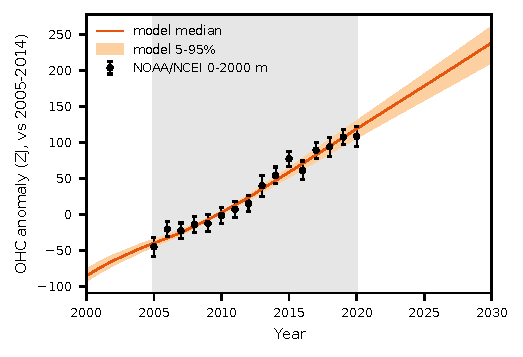
\includegraphics[width=0.6\textwidth]{figures/ohc_fit.pdf}
\caption{Posterior ocean heat content (0--2000\,m) against NOAA/NCEI observations
over the 2005--2020 constraint window (RMSE $8.0$\,ZJ).}
\label{fig:ohc}
\end{figure}

\begin{figure}[h]
\centering
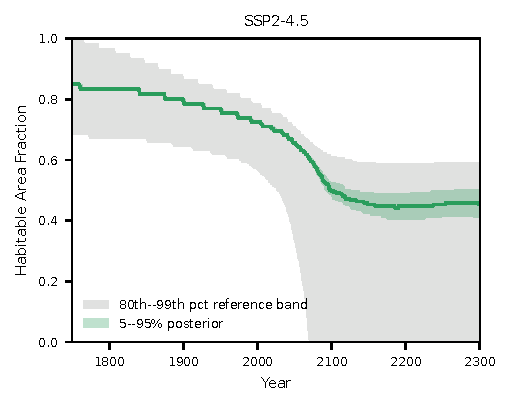
\includegraphics[width=0.6\textwidth]{figures/haf.pdf}
\caption{Headline (SSP2-4.5) HAF with the parametric posterior 5--95\% envelope and
the 80th--99th percentile threshold-sensitivity band.}
\label{fig:haf_band}
\end{figure}

\begin{figure}[h]
\centering
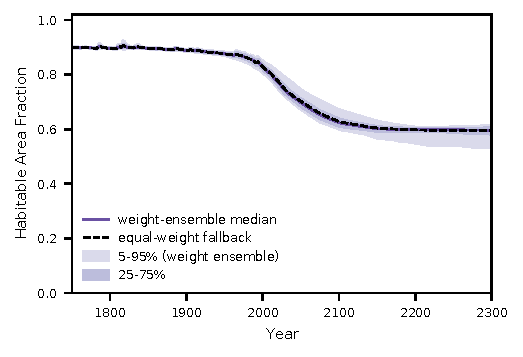
\includegraphics[width=0.6\textwidth]{figures/haf_weight_ensemble.pdf}
\caption{HAF under a flat-Dirichlet ensemble of $500$ six-variable weightings,
showing the small sensitivity of the HAF to the weighting choice (2100 5--95\%
width $0.072$).}
\label{fig:haf_weight}
\end{figure}

\begin{figure}[h]
\centering
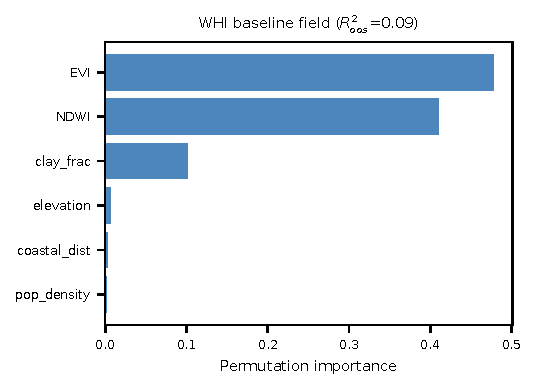
\includegraphics[width=0.6\textwidth]{figures/whi_rf_importances.pdf}
\caption{Descriptive Random-Forest permutation importances for the real gridded
Water Hazard Index, with the held-out $R^2$ on independent predictors and the
leakage when the WHI's own constituents are included. Illustrative only; not used
as CHS weights.}
\label{fig:rf}
\end{figure}

\bibliographystyle{unsrtnat}
\bibliography{references}

\end{document}
